\documentclass{article}
\usepackage[utf8]{inputenc}
\usepackage{natbib}
\usepackage{graphicx}

\title{IF689 - Informática Teórica}
\author{Júlio Vinícius Gonçalves dos Santos }
\date{November, 2019}

\begin{document}

\maketitle

\section{Introdução}
\quad Informática teoria é uma cadeira obrigatória do 4º período que aborda conceitos da teoria da computação, nessa disciplina é abordado assuntos como Definição de Algoritmos, Autômatos Finitos, Expressões regulares, Teoria da complexidade, podemos destacar o estudo das máquinas de Turing \citep{cinWiki} , a disciplina é lecionada pelo Prof. Ruy de Queiroz ou Prof. Fred Freitas.\citep{cinWiki2}

\begin{figure}[h!]
\centering
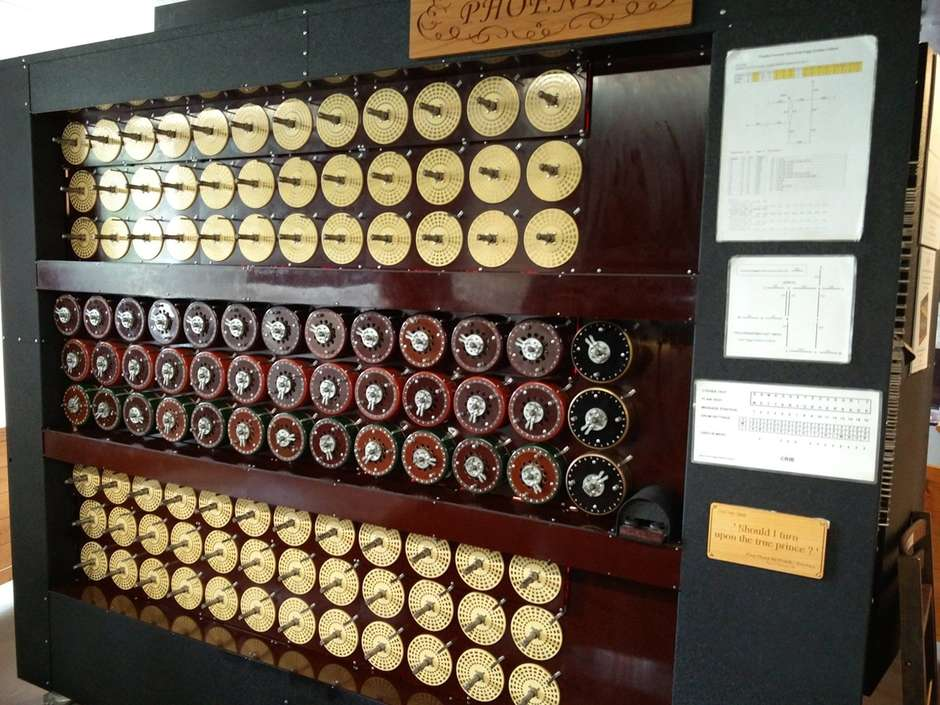
\includegraphics[scale=0.22]{Mturing}
\caption{máquina de turing. \cite{imagem}}
\end{figure}


\section{Relevância}
\quad Essa disciplina mostra conceitos teóricos importantes utilizados em outras disciplinas e áreas da computação, com isso os alunos terão base para inúmeras aplicações práticas da computação.
\section{Relação com outras disciplinas}
\quad A disciplina de Informática teoria possui como pré-requisito as disciplinas de Algoritmos e Estruturas de Dados e Lógica para computação e é pré-requisito de várias disciplinas, podemos destacar teoria da prova, teoria da recursão, teoria de grafos, teoria de modelos. \citep{ufpe}
\bibliographystyle{siam}
\bibliography{jvgs}
\end{document}
